\section{Evaluation}\label{sec:eval}
All numbers in this section are produced by scripts in the repository from the SF=0.05 run (about 1.3 million records, seed 42, 2021--2025) unless stated. The pipeline was afterwards re-run incrementally on a separate 14-day drop (Section~\ref{sec:drop}), so the quality counts and the forecast and allocation results use the history plus those two weeks, while detection is evaluated on the history only; the machine was one virtual CPU with 4~GB of memory.

\subsection{Outbreak detection (AN-2, AN-3)}
Detection is scored against the ground-truth file, which the detection code never reads. The first 14 months provide baseline history for the seasonal detector, so all methods are evaluated on the common period starting @@EVAL_START@@, which contains @@N_EVENTS@@ injected outbreak events (district by disease; the nationwide surge counts once per district). An event is detected if an alert episode overlaps the outbreak window extended by one week; an alert episode with no overlap with any true outbreak of the same district and disease (tolerance one week before and two after) is a false alert; the false alert rate is episodes per district-year over all diseases. Table~\ref{tab:det} gives the best admissible threshold of each method under the limit of one false alert episode per district-year, and Fig.~\ref{fig:det} shows the full trade-off.
@@DET_TABLE@@
\begin{figure}[t]\centering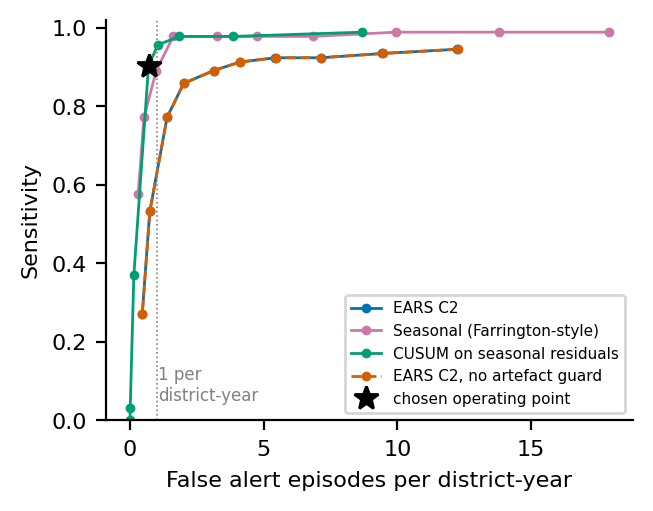
\includegraphics[width=0.9\columnwidth]{figures/detection_tradeoff.png}\caption{Detection trade-off (conflict C1): sensitivity against false alert episodes per district-year for threshold sweeps. The star marks the operating point.}\label{fig:det}\end{figure}
@@DET_TEXT@@

\subsection{Forecasting backtest (AN-5)}
The rolling-origin backtest covers the last 52 forecastable origins for dengue, diarrhoeal disease and malaria (64 districts, four horizons, 119\,808 forecast rows per model family), refitting every four origins and using only data mature at each origin. Targets are final onset-week counts. Table~\ref{tab:fc} reports the mean absolute error (MAE), the 80\% and 95\% prediction interval coverage and the weighted interval score (WIS~\cite{bracher}, with a median and 80\% and 95\% intervals) for the regression with weather, the same regression without weather, and the seasonal-naive baseline (the count of the same week one year earlier, with intervals from the same dispersion).
@@FC_TABLE@@
@@FC_TEXT@@
\begin{figure*}[t]\centering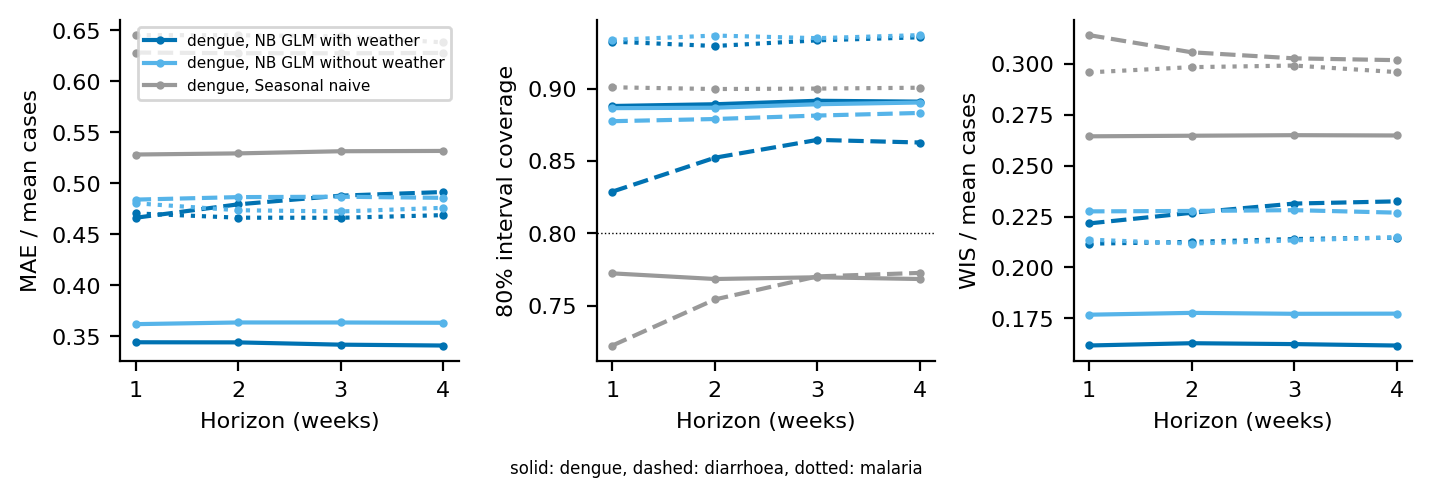
\includegraphics[width=\textwidth]{figures/forecast_backtest.png}\caption{Backtest by horizon: error relative to the mean observed count, 80\% interval coverage (dotted line is the nominal 80\%) and weighted interval score.}\label{fig:fc}\end{figure*}

\subsection{Allocation against the baseline (AN-7, AN-8)}
The planning scenario uses the forecast issued at the origin with the largest national need, the week of @@PLAN_ORIGIN@@, near the dengue peak; at the latest origin (@@LATEST_ORIGIN@@, low season) the national need is only USD @@LATEST_NEED@@, against USD @@PEAK_NEED@@ at the peak, so an allocation study there would be trivial. Stocks are those on hand at the origin week. Table~\ref{tab:alloc} compares the optimiser with the population-proportional split at a 60\% budget, and Fig.~\ref{fig:eq} shows the efficiency--equity curves for all five budgets.
@@ALLOC_TABLE@@
\begin{figure*}[t]\centering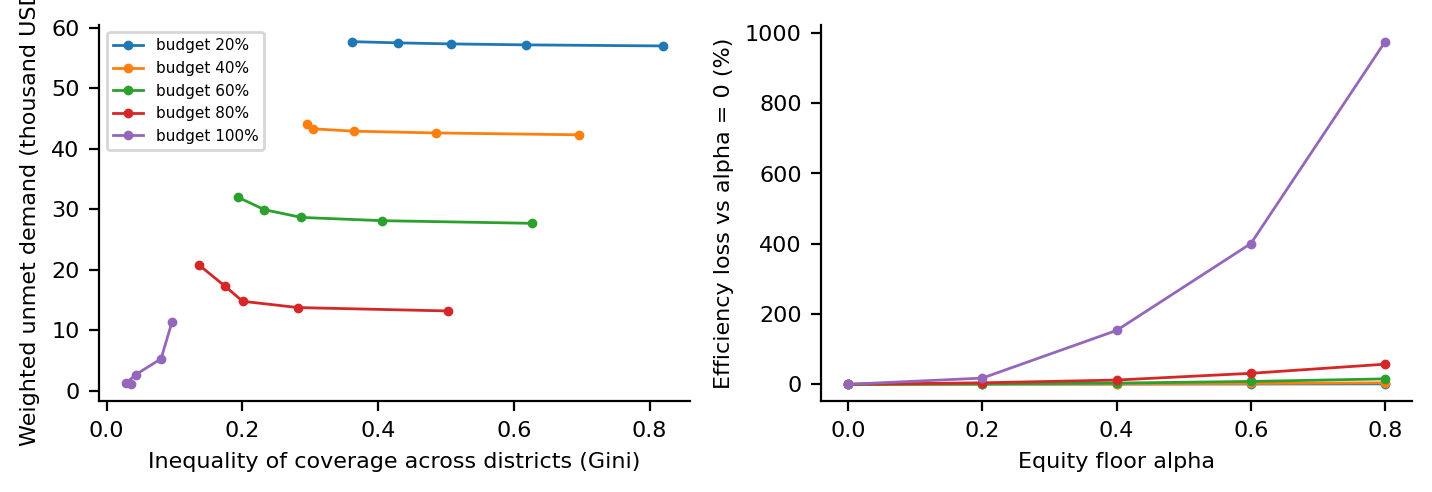
\includegraphics[width=0.8\textwidth]{figures/efficiency_equity.png}\caption{Efficiency--equity trade-off (conflict C3). Left: weighted unmet demand against inequality of coverage for $\alpha\in\{0,0.2,0.4,0.6,0.8\}$ (points along each line, left to right is more equal) and five budgets. Right: efficiency loss relative to $\alpha=0$.}\label{fig:eq}\end{figure*}
@@ALLOC_TEXT@@

\subsection{Scalability and Spark optimisations (ENG-2, ENG-3)}
@@SCALING_TEXT@@
@@OPT_TEXT@@

\subsection{Streaming path (ING-6) and tests (ENG-4)}
@@STREAM_TEXT@@
@@TEST_TEXT@@
